%! Author = gramic
%! Date = 22.03.24

% Preamble
\begin{flushleft}
    \subsubsection{Benchmark Settings}
    \label{subsubsec:benchmark_settings}
    Das Mass aller Dinge ist die Zabbix-DB.\\
    Sie wird vorerst die grössten Zugriffszahlen, das höchste Datenwachstum und die meisten Transaktionen erzeugen.\\
    Es werden alle Switches sowie der grösste Teil der Router erfasst, es sind im Moment etwas mehr als 32'000 Items erfasst.\\
    Ein Item kann ein Gerät, ein Port oder mehrere States pro Port sein:
    \begin{figure}[H]
        \centering
        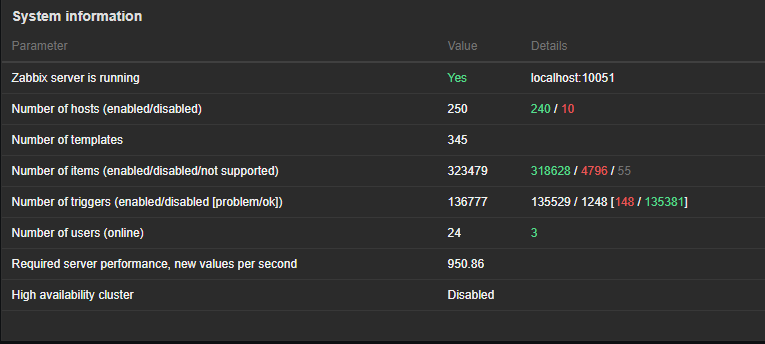
\includegraphics[width=0.8\linewidth]{source/implementation/evaluation/benchmarking/sks0970_zabbix_system_information}
        \caption{Benchmark Settings - Zabbix - Systeminformationen}
        \label{fig:sks0970_zabbix_system_information}
    \end{figure}
    Pro Sekunde werden ca.
    950 Datenpunkte abgeholt.
\end{flushleft}
\begin{flushleft}
    Da der grossteil der Netzwerksysteme aber erfasst sind, wird die Anzahl Items nicht mehr stark anwachsen.
\end{flushleft}
\begin{flushleft}
    Auf die Datenbank wird sehr stark zugegriffen.
    Es werden bis zu 23 Connections pro Sekunde ausgeführt:
    \begin{figure}[H]
        \centering
        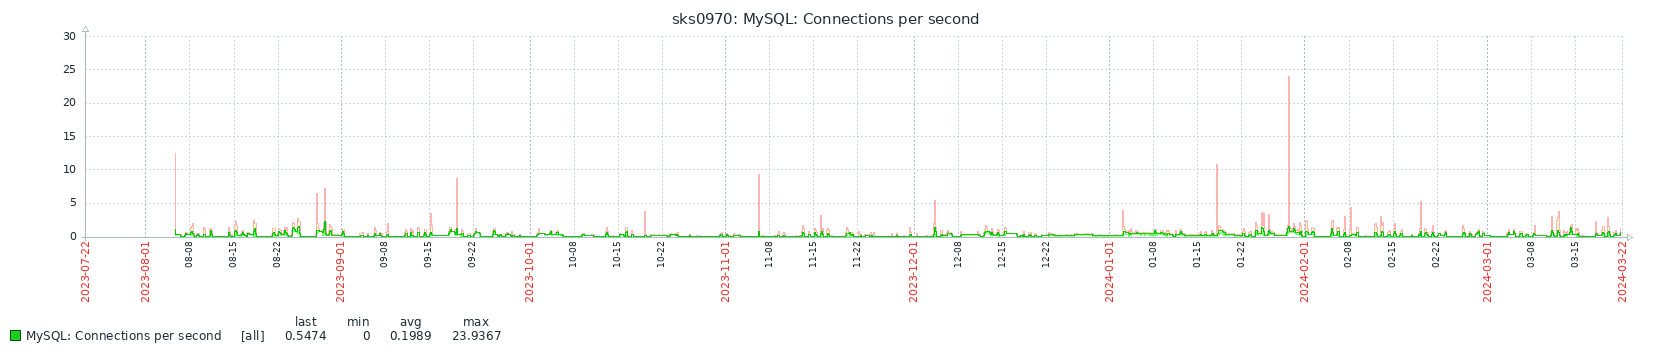
\includegraphics[width=0.8\linewidth]{source/implementation/evaluation/benchmarking/sks0970_zabbix_mariadb_connections_per_second_graph}
        \caption{Benchmark Settings - Zabbix - Connections per Seconds}
        \label{fig:sks0970_zabbix_mariadb_connections_per_second_graph}
    \end{figure}
\end{flushleft}
\begin{flushleft}
    Pro Sekunde wurden bisher bis zu über 7'000 Queries ausgeführt.
    Dies schliesst Abfragen von Stored Programs ein:
    \begin{figure}[H]
        \centering
        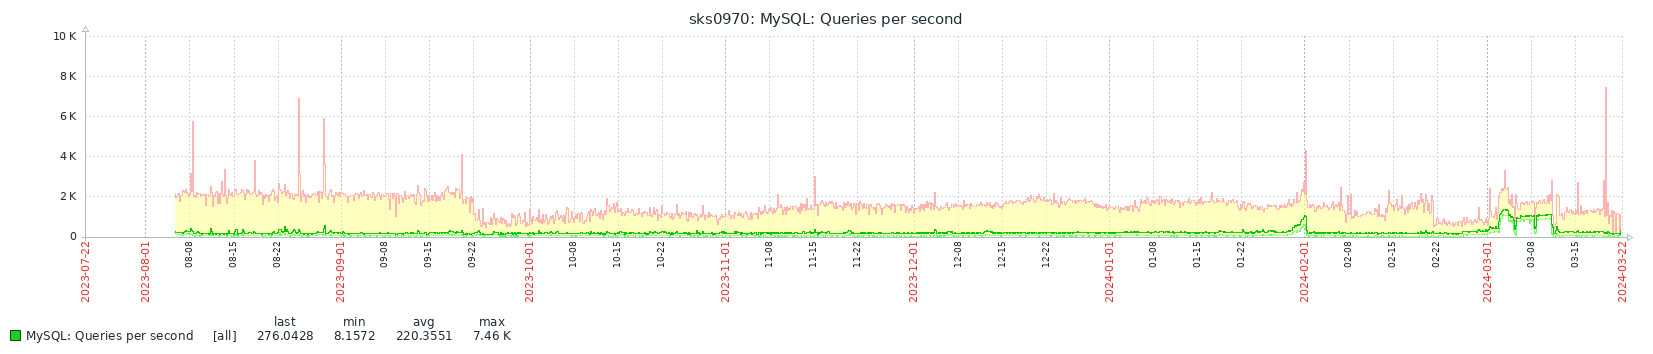
\includegraphics[width=0.8\linewidth]{source/implementation/evaluation/benchmarking/sks0970_zabbix_mariadb_queries_per_second_graph}
        \caption{Benchmark Settings - Zabbix - Queries per Seconds}
        \label{fig:sks0970_zabbix_mariadb_queries_per_second_graph}
    \end{figure}
    Reine Client anfragen waren nichtsdestotrotz über 4'000 Queries pro Sekunde:
    \begin{figure}[H]
        \centering
        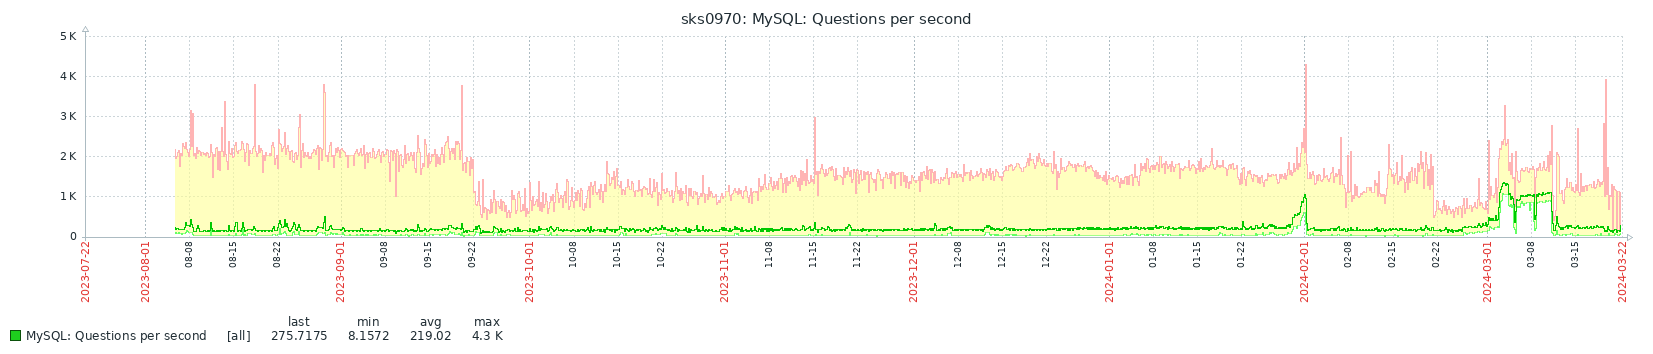
\includegraphics[width=0.8\linewidth]{source/implementation/evaluation/benchmarking/sks0970_zabbix_mariadb_questions_per_second_graph}
        \caption{Benchmark Settings - Zabbix - Client Queries per Seconds}
        \label{fig:sks0970_zabbix_mariadb_questions_per_second_graph}
    \end{figure}
\end{flushleft}
\begin{flushleft}
    Auch das wachstum ist beachtlich.
    Die DB startete mit 180GiB und ist zurzeit bei rund 232GiB, war aber schon bei 238GiB:
    \begin{figure}[H]
        \centering
        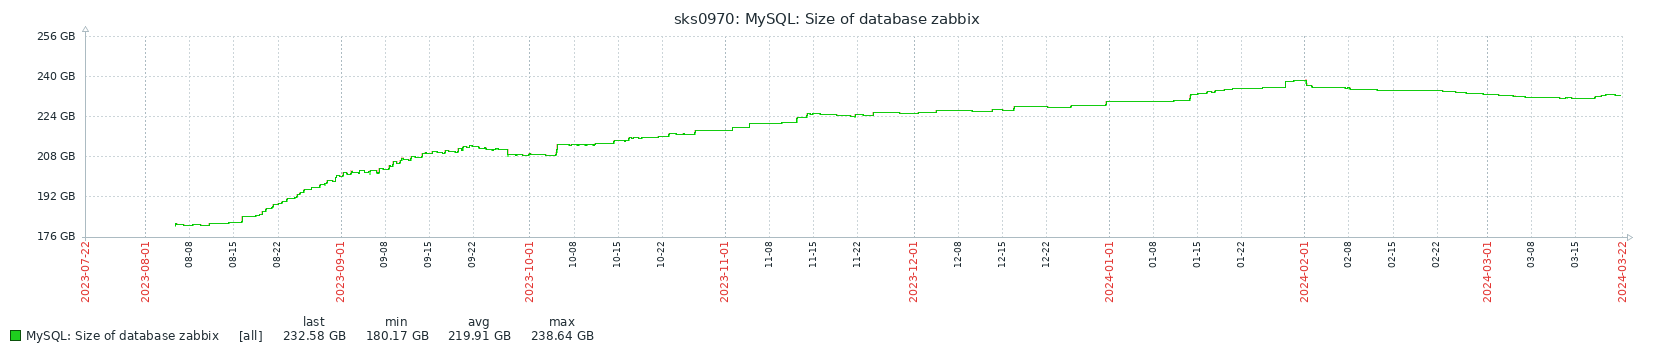
\includegraphics[width=0.8\linewidth]{source/implementation/evaluation/benchmarking/sks0970_zabbix_mariadb_size_graph}
        \caption{Benchmark Settings - Zabbix - DB Size}
        \label{fig:sks0970_zabbix_mariadb_size_graph}
    \end{figure}
\end{flushleft}
\begin{flushleft}
    Nun kommen noch die restlichen, kleineren DBs hinzu.
    Heisst, für den Mixed Benchmark (DML und DQL \Gls{Transaktion}en) werden folgende Werte und Parameter gesetzt:
    \begin{table}[H]

\resizebox{\columnwidth}{!}{%

\begin{tabular}{lllllll}
\toprule
Typ & Parameter & pgbench-Parameter & 1. Lauf & 2. Lauf & 3. Lauf & 4. Lauf \\
\midrule
mixed & Datenbank &  & pgbench\_eval\_bench & pgbench\_eval\_bench & pgbench\_eval\_bench & pgbench\_eval\_bench \\
mixed & DB-Grösse &  & 5GiB & 15GiB & 50GiB & 250GiB \\
mixed & 1. Iteration Lauf ignorieren &  & ja & ja & ja & ja \\
mixed & Select only & -S & nein & nein & nein & nein \\
mixed & Iterationen pro Lauf &  & 4 & 4 & 4 & 4 \\
mixed & Vacuum & -v & ja & ja & ja & ja \\
mixed & Separate Connects & -C & ja & ja & ja & ja \\
mixed & Client count & -c & 10 & 50 & 100 & 1000 \\
mixed & Anzahl Transaktionen pro Client & -t & 10 & 50 & 1000 & 7000 \\
mixed & Anzahl Worker Threads & -j & 4 & 4 & 4 & 4 \\
\bottomrule
\end{tabular}
}
\caption{Benchmark Settings - Mixed Transaktionen} \label{benchmarking_settings_mixed}
\end{table}

\end{flushleft}
\begin{flushleft}
    Für den DQL-Only Benchmark wird mit folgenden Konfigurationen gearbeitet:
    \begin{table}[H]

\resizebox{\columnwidth}{!}{%

\begin{tabular}{lllllll}
\toprule
Typ & Parameter & pgbench-Parameter & 1. Lauf & 2. Lauf & 3. Lauf & 4. Lauf \\
\midrule
dql & Datenbank &  & pgbench\_eval\_bench & pgbench\_eval\_bench & pgbench\_eval\_bench & pgbench\_eval\_bench \\
dql & DB-Grösse &  & 5GiB & 15GiB & 50GiB & 250GiB \\
dql & 1. Iteration Lauf ignorieren &  & ja & ja & ja & ja \\
dql & Select only & -S & ja & ja & ja & ja \\
dql & Iterationen pro Lauf &  & 4 & 4 & 4 & 4 \\
dql & Vacuum & -v & ja & ja & ja & ja \\
dql & Separate Connects & -C & ja & ja & ja & ja \\
dql & Client count & -c & 10 & 50 & 100 & 1000 \\
dql & Anzahl Transaktionen pro Client & -t & 10 & 50 & 50 & 7 \\
dql & Anzahl Worker Threads & -j & 4 & 4 & 4 & 4 \\
\bottomrule
\end{tabular}
}
\caption{Benchmark Settings - DQL Transaktionen} \label{benchmarking_settings_dql}
\end{table}

\end{flushleft}
\begin{flushleft}
    Bei \texttt{pgbench} kann nicht einfach die grösse angegeben werden.\\
    Es muss der Skalierungsfaktor angepasst werden.\\
    Dieser legt allerdings fest, wie viele Daten gespeichert werden.\\
    Wird eine \texttt{1} eingeben, so werden \texttt{100'000} Records angelegt.\\

    Um nun auf eine gewisse grösse zu kommen, gibt es verschiedene Formeln.\\
    Die als beste stellte sich folgende heraus\cite{DKXU3QRC}:\\
    \begin{table}[H]

\resizebox{\columnwidth}{!}{%

\begin{tabular}{ll}
\toprule
Zielobjekt & Skalierungsfaktor Formel \\
\midrule
DB & 0.0669 * DB-Zielgrösse -0.5 \\
Tabelle (pgbench\_accounts / ysql\_bench\_accounts) & \(0.0781 * Tabelle-Zielgrösse\) \\
Index (pgbench\_accounts\_pkey / ysql\_bench\_accounts\_pkey) & \(0.4668 * Index-Zielgrösse\) \\
\bottomrule
\end{tabular}
}
\caption{Benchmark Settings - Skalierungsfaktoren} \label{benchmarking_formeln}
\end{table}

\end{flushleft}
\begin{flushleft}
    Daraus errechnen sich für die DB-Grössen des Benchmark-Settings folgende skalierungsfaktoren:\\
    \begin{table}[H]

\resizebox{\columnwidth}{!}{%

\begin{tabular}{rrr}
\toprule
DB Grösse [GiB] & DB Grösse [MiB] & Scale Faktor \\
\midrule
5 & 5120 & 342 \\
15 & 15360 & 1027 \\
50 & 51200 & 3425 \\
250 & 256000 & 17126 \\
\bottomrule
\end{tabular}
}
\caption{Benchmark Settings - Datenbankgrössen / Skalierungsfaktor} \label{benchmarking_db_sizes}
\end{table}

\end{flushleft}
\begin{flushleft}
    yugabyteDB speichert die Daten anders als PostgreSQL, nämlich als \Gls{Key-Value-Store}.\\
    Das verhindert, dass die DB Grösse nicht ausgelesen werden kann, nur die Tabellen sind ersichtlich.\\
    Um einen Vergleich zu haben, muss daher die Tabellengrösse berechnet werden.\\
    Der skalierungsfaktor für die Tabellen ist folgendermassen aufgebaut:\\
    {\small
\begin{table}[H]

\resizebox{\columnwidth}{!}{%

\begin{tabular}{rrr}
\toprule
DB Grösse [GiB] & DB Grösse [MiB] & Scale Faktor \\
\midrule
5 & 5120 & 400 \\
15 & 15360 & 1200 \\
50 & 51200 & 3999 \\
250 & 256000 & 19994 \\
\bottomrule
\end{tabular}
}
\caption{Benchmark Settings - Tabellenvolumen / Skalierungsfaktor} \label{benchmarking_table_sizes}
\end{table}

}
\end{flushleft}
\begin{flushleft}
    Der Skalierungsfaktor wird pro 100'000 gerechnet, gebe ich also den Faktor 1 ein, werden 100'000 Zeilen in der Tabelle \texttt{pgbench\_accounts} resp. \texttt{ysql\_bench\_accounts} erzeugt.\\
    Entsprechend wachsen die Anzahl Records wie folgt an:\\
    \begin{figure}[H]
        \centering
        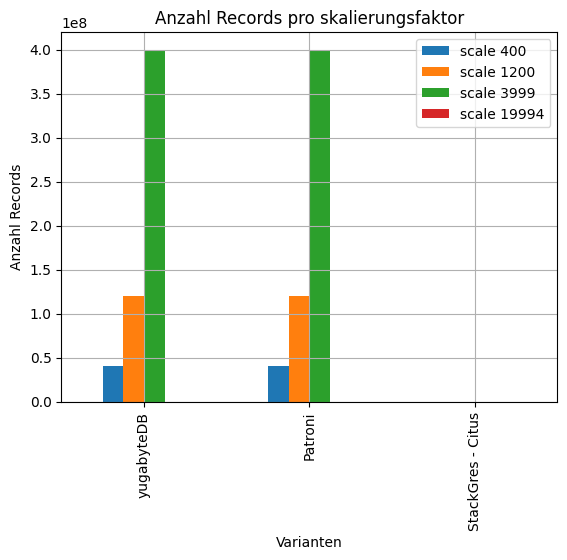
\includegraphics[width=0.8\linewidth]{source/pandas_data_chart_plotter/row_counts}
        \caption{Benchmark Settings - Anzahl Records / Skalierungsfaktor}
        \label{fig:row_counts}
    \end{figure}
\end{flushleft}